\documentclass{article}

\usepackage{amsmath}
\usepackage{listings}
\usepackage{graphicx}
\usepackage{xcolor}

\definecolor{codegreen}{rgb}{0,0.6,0}
\definecolor{codegray}{rgb}{0.5,0.5,0.5}
\definecolor{codepurple}{rgb}{0.58,0,0.82}
\definecolor{backcolour}{rgb}{0.95,0.95,0.92}

\lstdefinestyle{mystyle}{
    backgroundcolor=\color{backcolour},   
    commentstyle=\color{codegreen},
    keywordstyle=\color{magenta},
    numberstyle=\tiny\color{codegray},
    stringstyle=\color{codepurple},
    basicstyle=\ttfamily\footnotesize,
    breakatwhitespace=false,         
    breaklines=true,                 
    captionpos=b,                    
    keepspaces=true,                 
    numbers=left,                    
    numbersep=5pt,                  
    showspaces=false,                
    showstringspaces=false,
    showtabs=false,                  
    tabsize=2
}

\lstset{style=mystyle}

\begin{document}

\begin{titlepage}
\begin{center}
\vspace*{1cm}
		
\textbf{Lab 2}
			
\vspace{0.5cm}
Chengxuan Li
			
\vspace{0.1cm}
1631060
			
\vspace{0.1cm}
Section 801
			
\vspace{0.1cm}
Oct 19th, 2021
\end{center}
\end{titlepage}

\section{Convolution}

\begin{enumerate}
\item[Q1(a)] Plot of two given function and Matlab script.

\begin{lstlisting}[language=Matlab]
k = (0:1:4);
x = k;
h = zeros(1,4) + 2 - k(1:4);

tiledlayout(2,1);
ax1 = nexttile;
stem(ax1, k, x);
title('Plot of x[k]', 'Fontsize', 16);
xlabel('k', 'Fontsize', 16);
ylabel('x[k]', 'Fontsize', 16);

ax2 = nexttile;
stem(ax2, k(1:4), h);
title('Plot of h[k]', 'Fontsize', 16);
xlabel('k', 'Fontsize', 16);
ylabel('h[k]', 'Fontsize', 16);
\end{lstlisting}

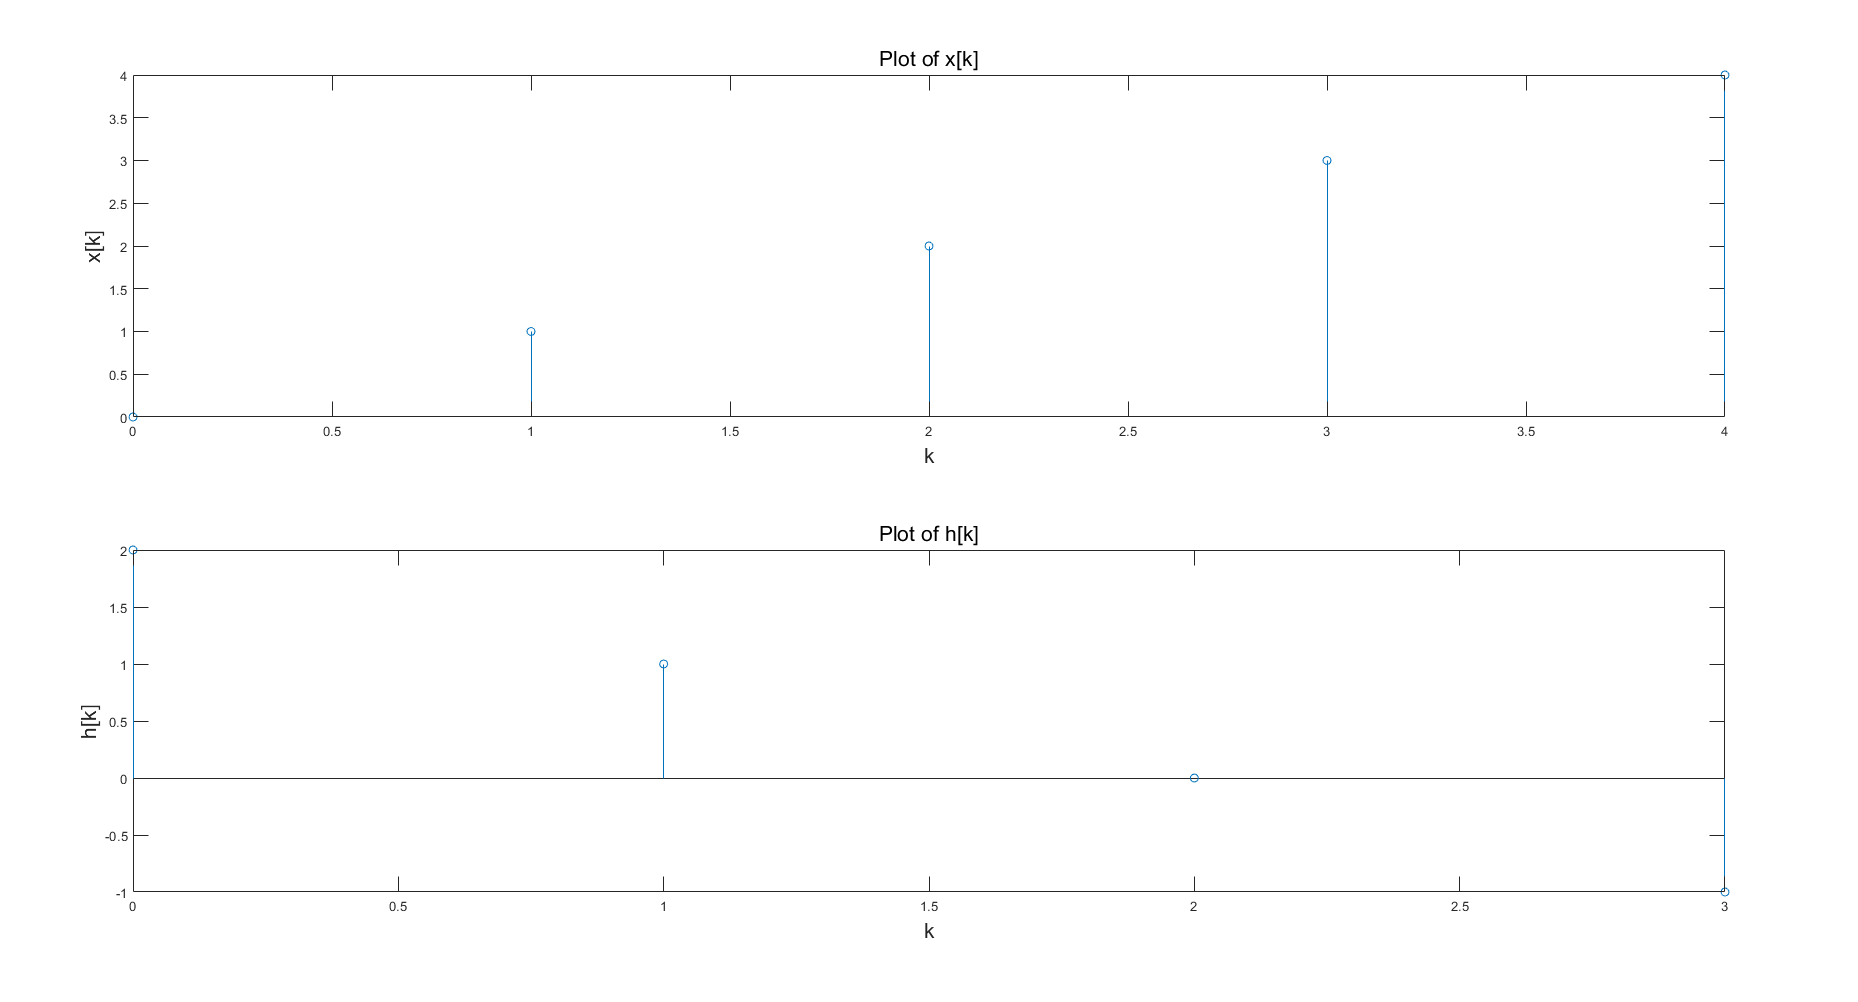
\includegraphics[width=\textwidth]{Question1A.png}

\item[Q1(b)] Plot of the convolution results and MATLAB script.

\begin{lstlisting}[language=Matlab]
xh = conv(h, x);
tiledlayout(1,1);
stem(xh);
title('Plot of  convolution output', 'Fontsize', 16);
xlabel('k', 'Fontsize', 16);
ylabel('x[k] * h[k]', 'Fontsize', 16);
\end{lstlisting}

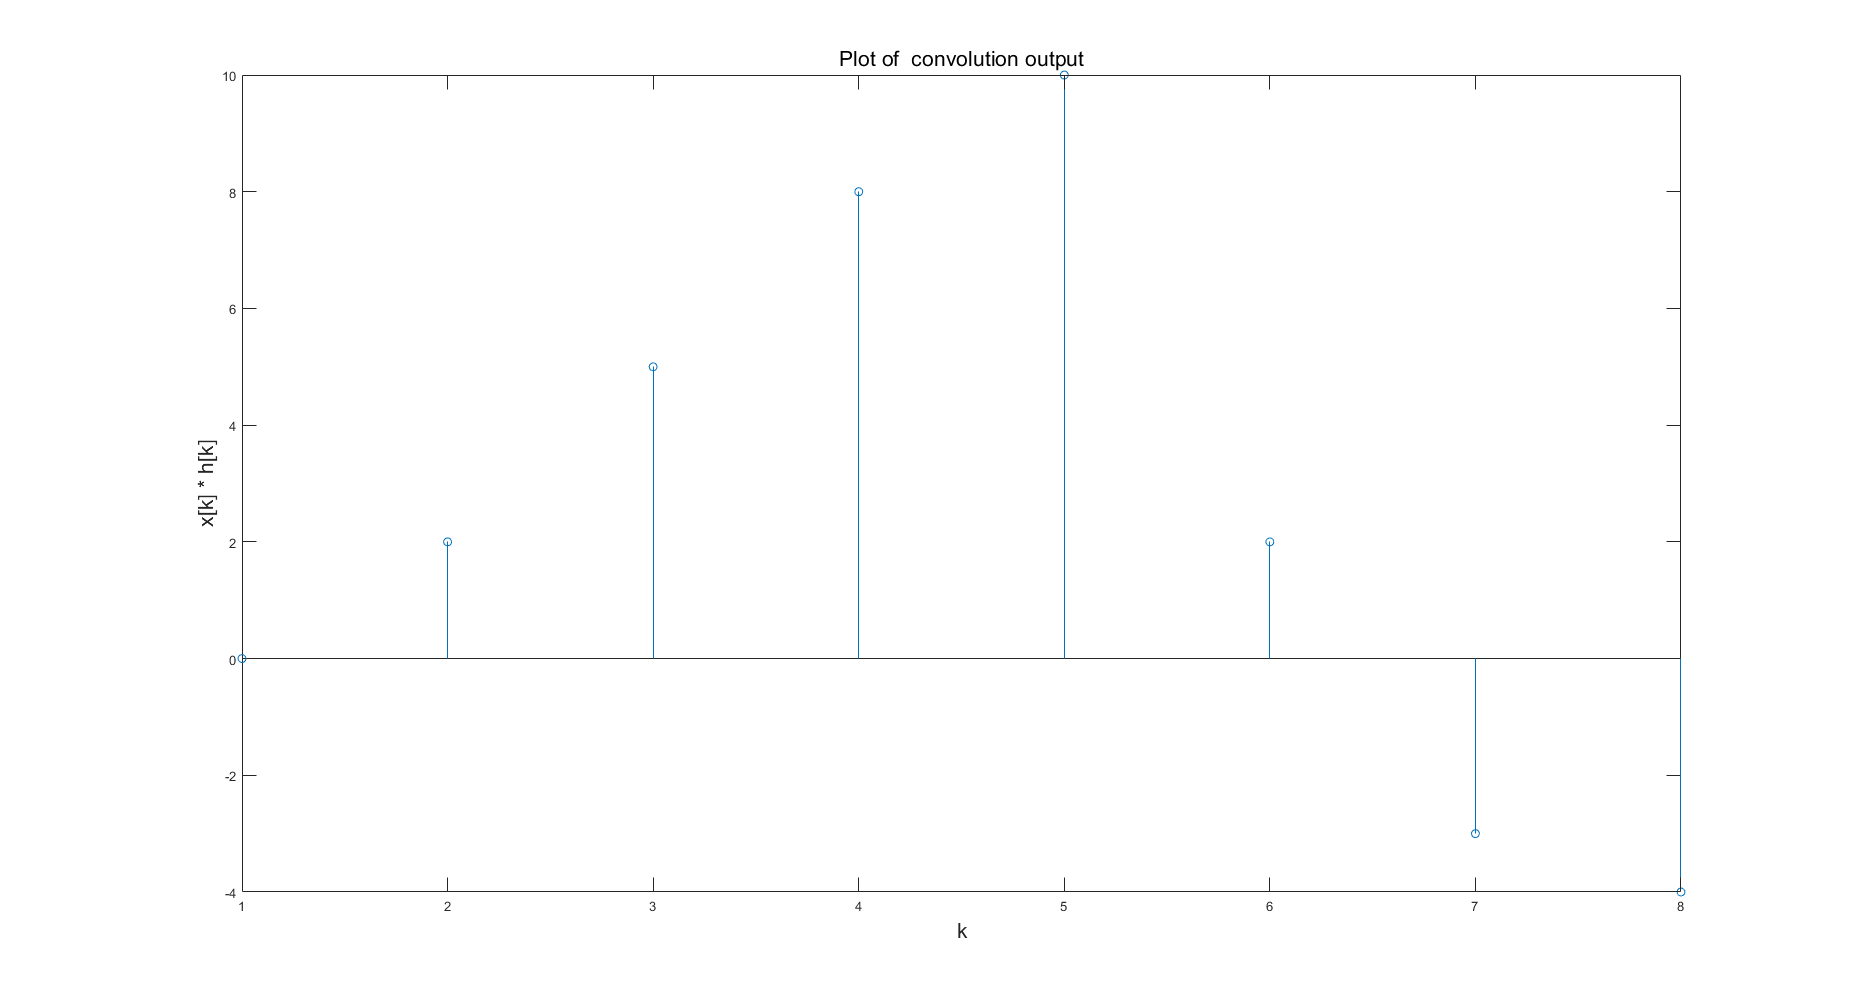
\includegraphics[width=\textwidth]{Question1B.png}

\item[Q1(d)] Verify the results of part c using sliding tap method in Excel.

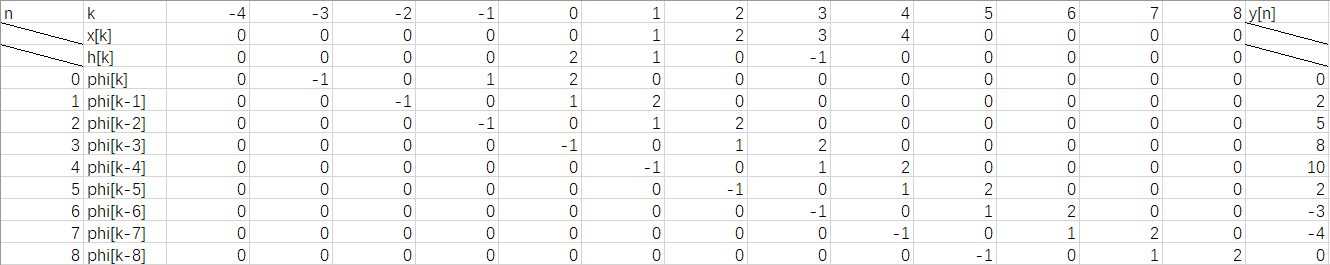
\includegraphics[width=\textwidth]{Question1CExcel.png}

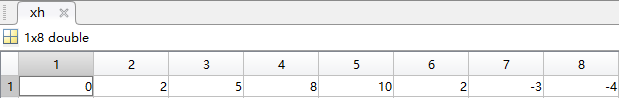
\includegraphics[width=\textwidth]{Question1CMatlab.png}

\end{enumerate}

\section{Convolution}

\begin{enumerate}
\item[Q2(b)] Plot of the h[k] and MTLAB script.

\begin{lstlisting}[language=Matlab]
k = (0:1:50);
sincPart = 0.3 .* sinc(0.3 .* (k - 25));
cosPart = 0.54 - 0.46 .* cos(2 .* pi .* k ./ 50 );
h = sincPart .* cosPart;

stem(h);
title('Plot of h[k]', 'Fontsize', 16);
xlabel('k', 'Fontsize', 16);
ylabel('h[k]', 'Fontsize', 16);
\end{lstlisting}

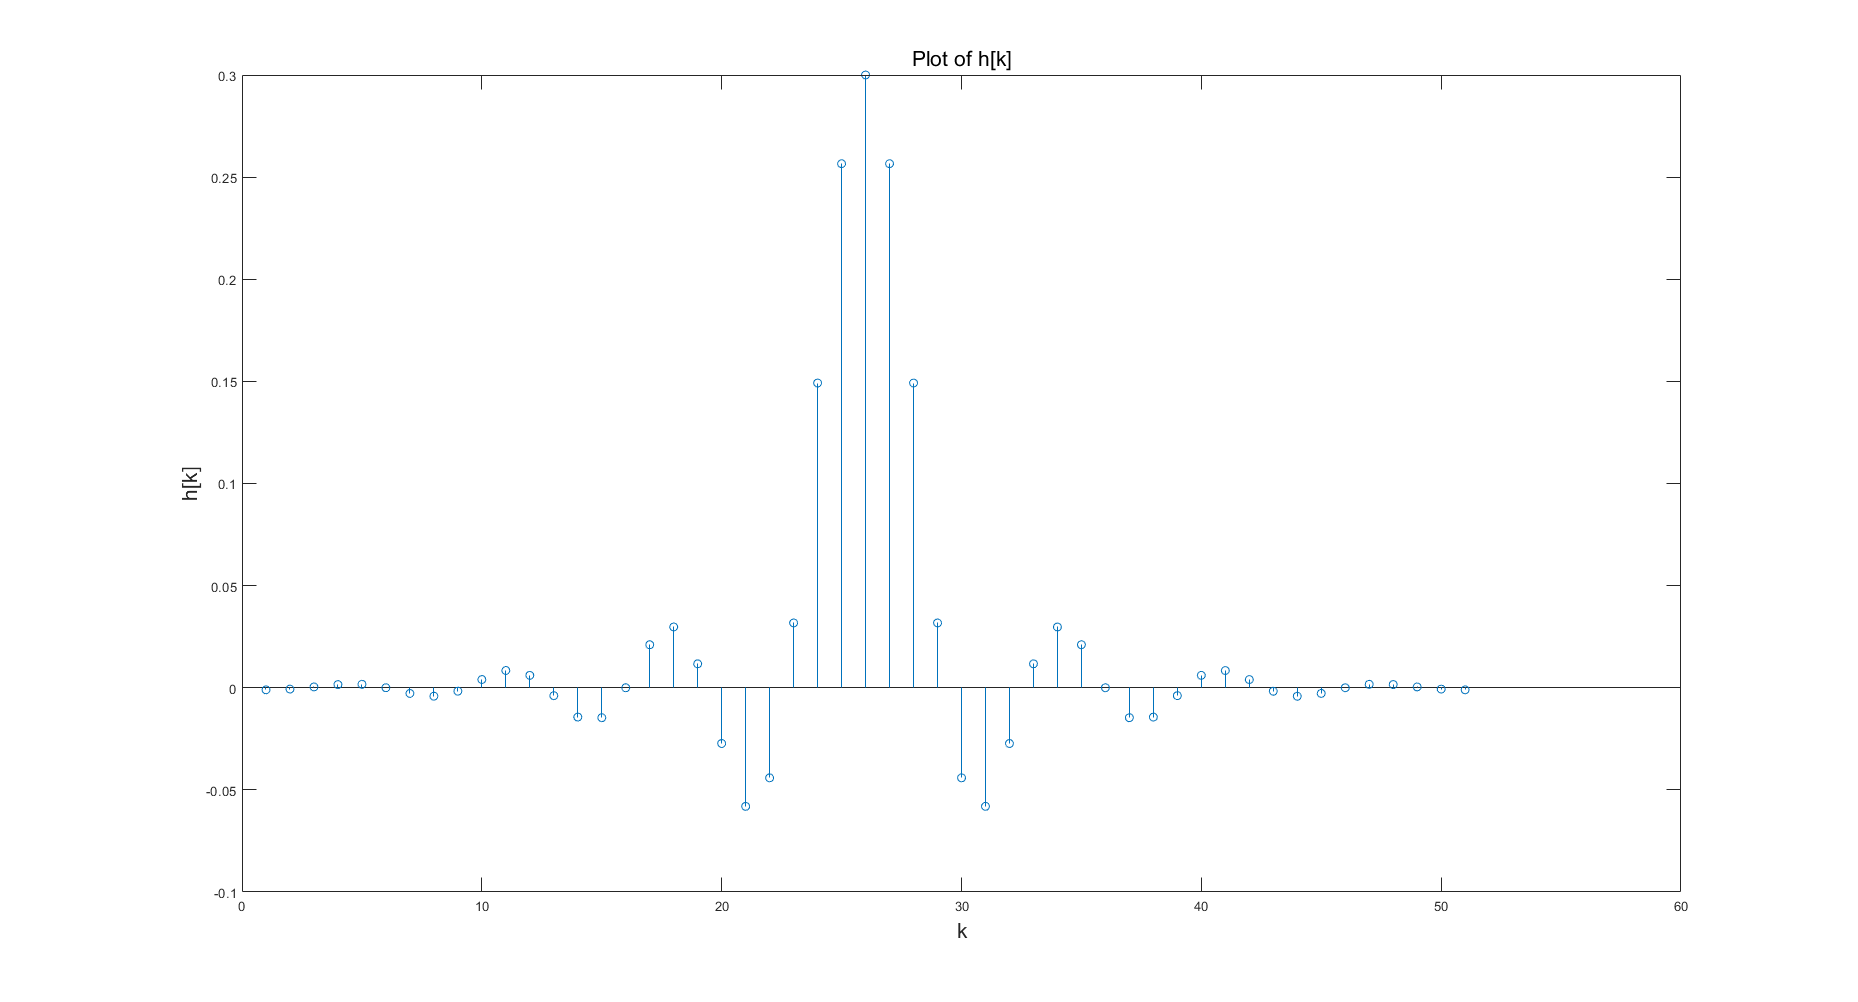
\includegraphics[width=\textwidth]{Question2B.png}

\item[Q2(c)] MATLAB script for calculating the convolution results
\begin{lstlisting}[language=Matlab]
[x3, Fs] = audioread("baila.wav");
x3h = conv(x3, h);
\end{lstlisting}

\item[Q2(d)] MATLAB script for store the convolution output as \textbf{baila\_filtered.wav} 

\begin{lstlisting}[language=Matlab]
audiowrite("baila_filtered.wav", x3h, Fs);
\end{lstlisting}

\item[Q2(e)] The audio quality of the filtered version was distincly lower than the 
original version. Specially, the instrucment, which creates medium to relative high
 frequency (pitch) sound, became less clear and more dull in the audio due to sink 
 function in $h[k]$.

\end{enumerate}

\section{Aliasing effects on 1D sinusoidal signals}

\begin{enumerate}
\item[Q3(a)] Plot of y1[n] and y2[n], and MATLAB script. The sample version of 
both sinusoids were identical.

\begin{lstlisting}
n1 = (0:1:30);
fs1 = 100;
y1 = cos(20 .* pi .* n1 ./ fs1);
y2 = cos(180 .* pi .* n1 ./ fs1);
    
tiledlayout(2,1);
ax1 = nexttile;
stem(ax1, n1, y1);
title('Plot of y1[n]', 'Fontsize', 16);
xlabel('n', 'Fontsize', 16);
ylabel('y1[n]', 'Fontsize', 16);
ax2 = nexttile;
stem(ax2, n1, y2);
title('Plot of y2[n]', 'Fontsize', 16);
xlabel('n', 'Fontsize', 16);
ylabel('y2[n]', 'Fontsize', 16);
\end{lstlisting}

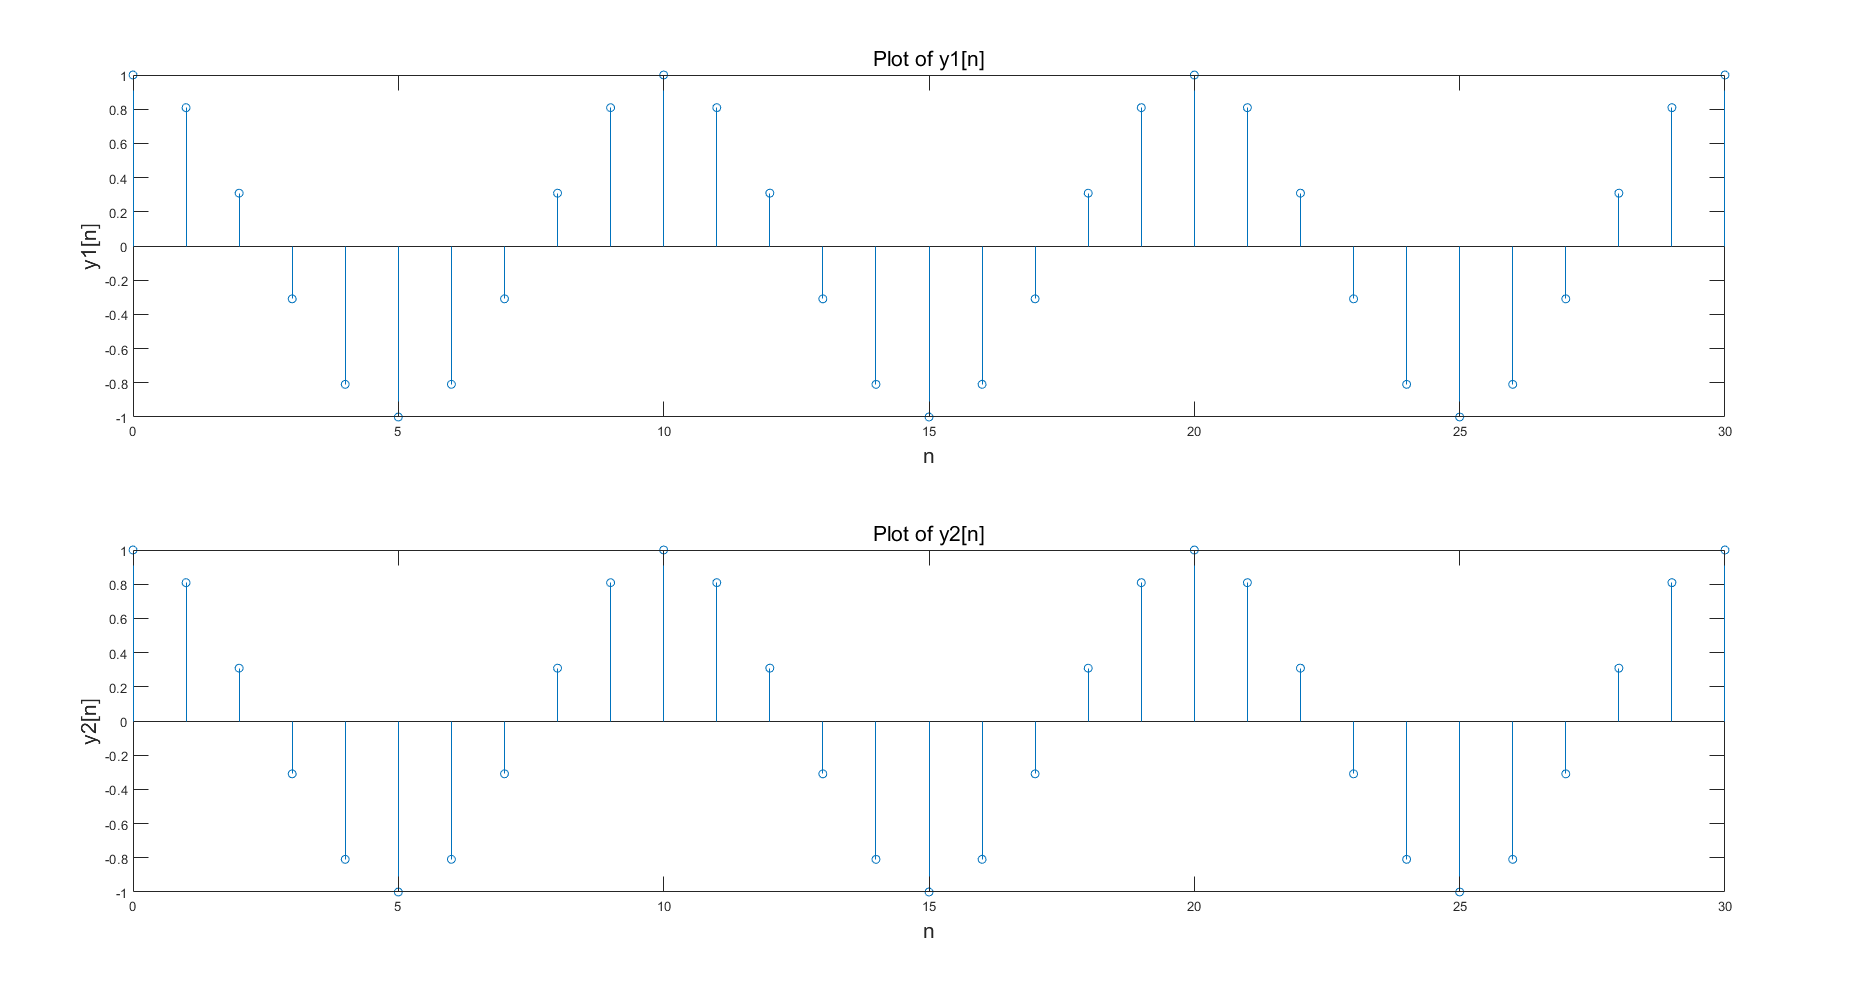
\includegraphics[width=\textwidth]{Question3A.png}

\item[Q3(b)] Plot of z1[n] and z2[n], and MATLAB script. The plot of z1[n] and 
z2[n] were clearly distinguishable after increasing the sampling frequency. By 
increasing the sample frequency, which were two times larger than the frequency 
of the x1[n] and x2[n],the number of samples increased. Thus, after converting 
these samples back to continuous time signals, which corresponds to z1[n] and 
z2[n] respectively, z1[n] and z2[n] were more accurate and close to what x1[n] 
and x2[n]. Compared to the sample frequency used for y1[n] and y2[n], y1[n] and 
and z1[n] were both accurate because the sample frequency was high enough to take 
more samples, which prevent that one sample and its aliasing become indistinguishable
to each other. For y2[n], the sample frequency was smaller than the frequency of x2[n].
Thus, it took less samples, and it created inaccuracy reconstruction because of 
overlapping with one sample and its aliasing. 

\begin{lstlisting}
n2 = (0:1:300);
fs2 = 1000;
z1 = cos(20 .* pi .* n2 ./ fs2);
z2 = cos(180 .* pi .* n2 ./ fs2);
    
tiledlayout(2,1);
ax1 = nexttile;
stem(ax1, n2, z1);
title('Plot of z1[n]', 'Fontsize', 16);
xlabel('n', 'Fontsize', 16);
ylabel('z1[n]', 'Fontsize', 16);
ax2 = nexttile;
stem(ax2, n2, z2);
title('Plot of z2[n]', 'Fontsize', 16);
xlabel('n', 'Fontsize', 16);
ylabel('z2[n]', 'Fontsize', 16);

subplot(2,1,1);
plot(n2/fs2,z1,'r-', n1/fs1,y1,'b+'); 
xlabel('n'); ylabel('y_1[n] and z_1[n]'); 
legend('z_1[n]','y_1[n]');
subplot(2,1,2);
plot(n2/fs2,z2,'r-', n1/fs1,y2,'b+');
xlabel('n'); ylabel('y_2[n] and z_2[n]'); 
legend('z_2[n]','y_2[n]');
\end{lstlisting}

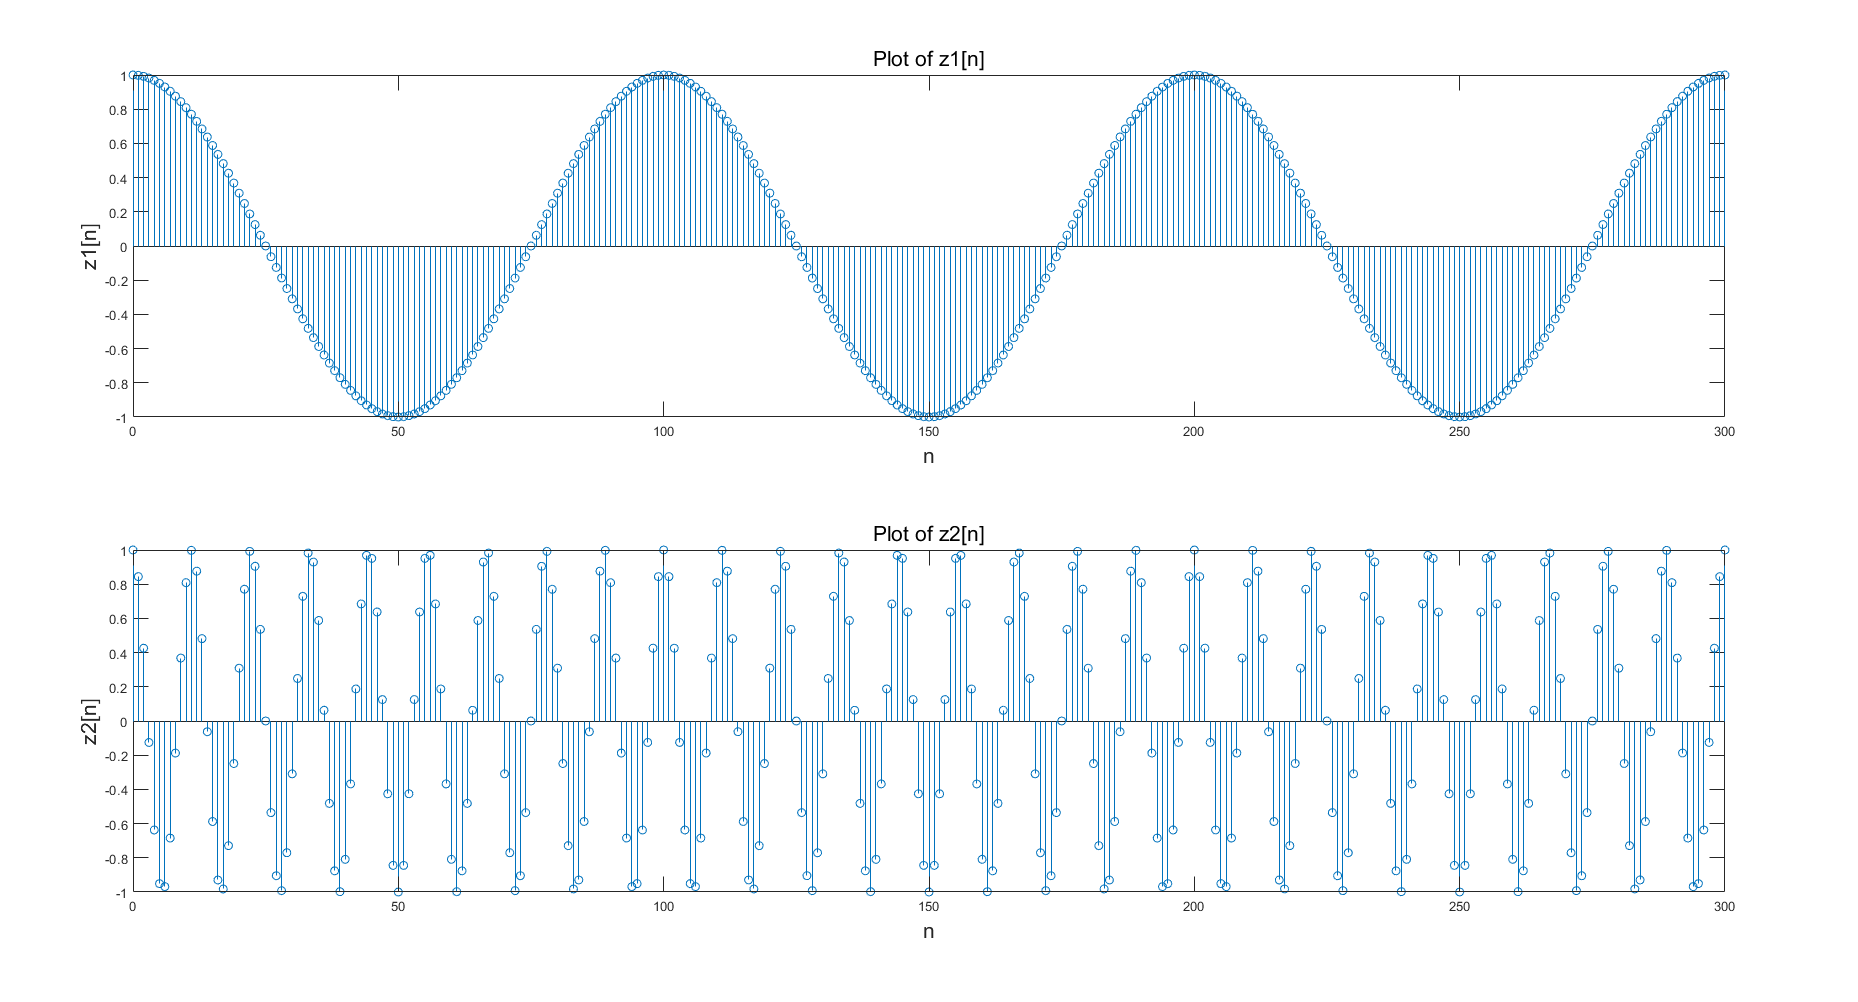
\includegraphics[width=\textwidth]{Question3B.png}

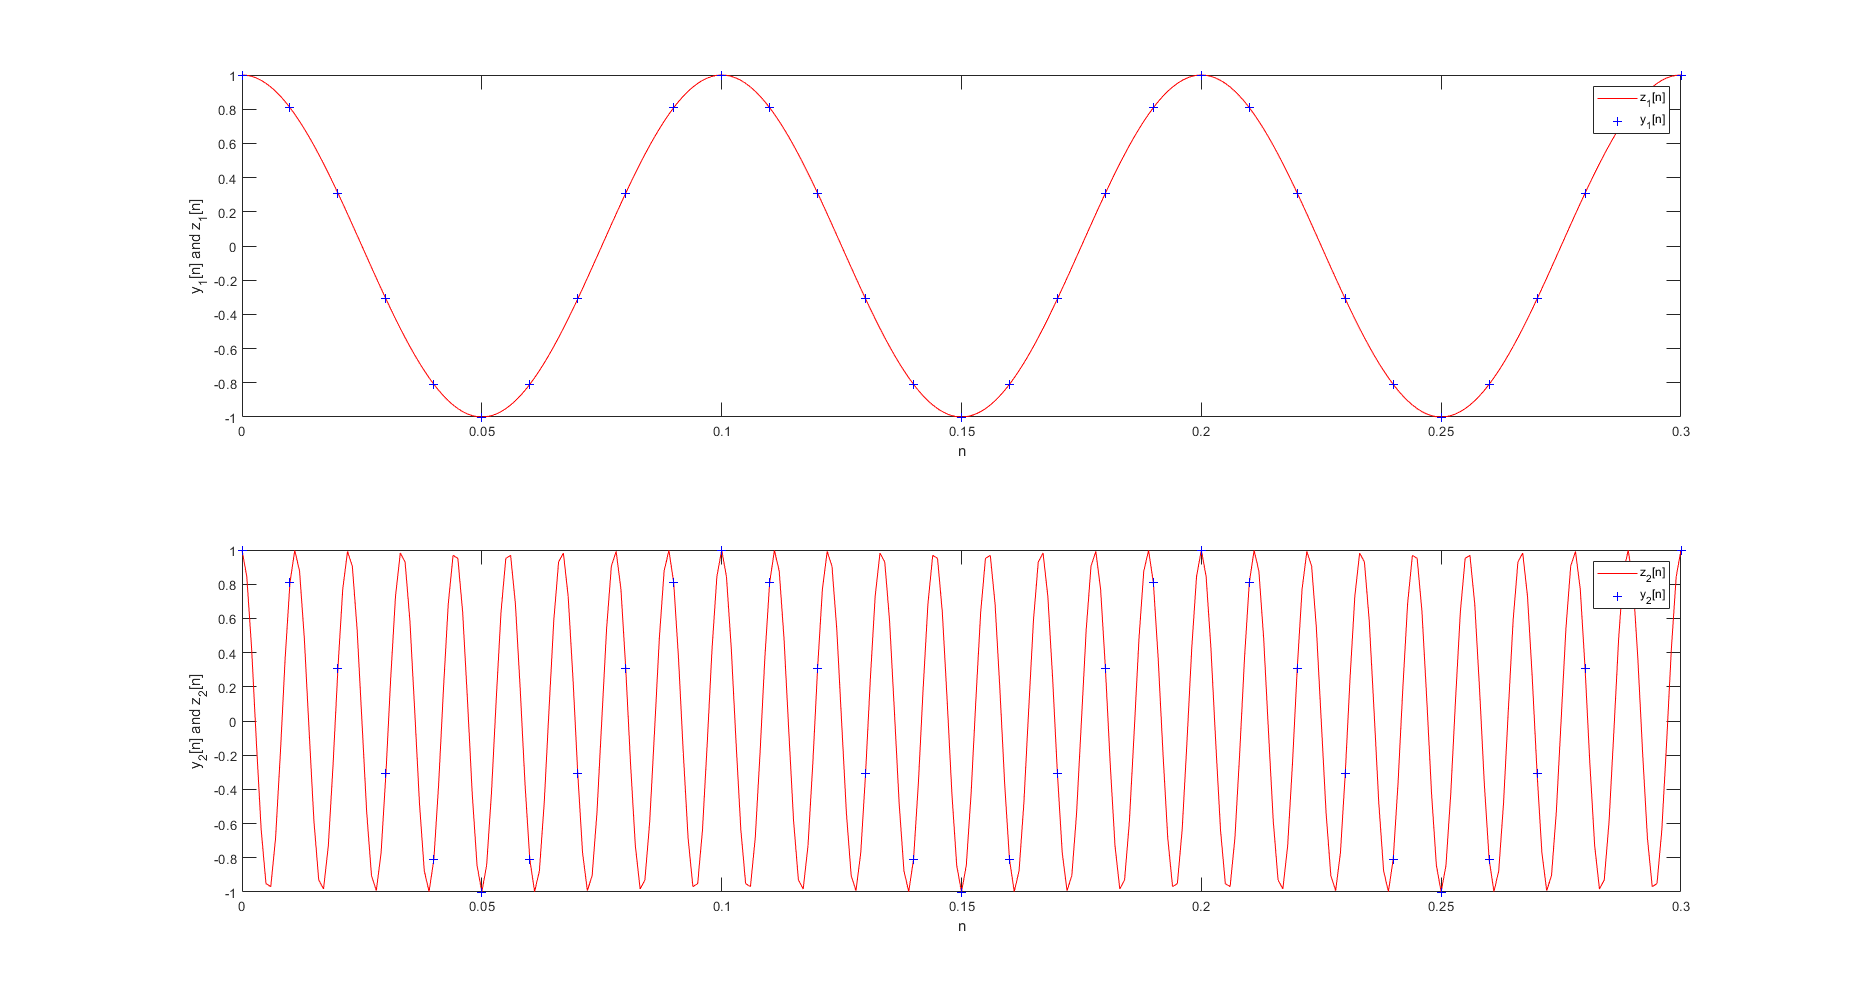
\includegraphics[width=\textwidth]{Question3BTest.png}

\item[Q3(c)] $x_3 = cos(220 \pi t)$. Plot of y1[n] and y3[n], and Matlab script.

\begin{lstlisting}[language=Matlab]
n1 = (0:1:30);
fs1 = 100;
y1 = cos(20 .* pi .* n1 ./ fs1);
y3 = cos(220 .* pi .* n1 ./ fs1);
    
tiledlayout(2,1);
ax1 = nexttile;
stem(ax1, n1, y1);
title('Plot of y1[n]', 'Fontsize', 16);
xlabel('n', 'Fontsize', 16);
ylabel('y1[n]', 'Fontsize', 16);
ax2 = nexttile;
stem(ax2, n1, y3);
title('Plot of y3[n]', 'Fontsize', 16);
xlabel('n', 'Fontsize', 16);
ylabel('y2[n]', 'Fontsize', 16);
\end{lstlisting}

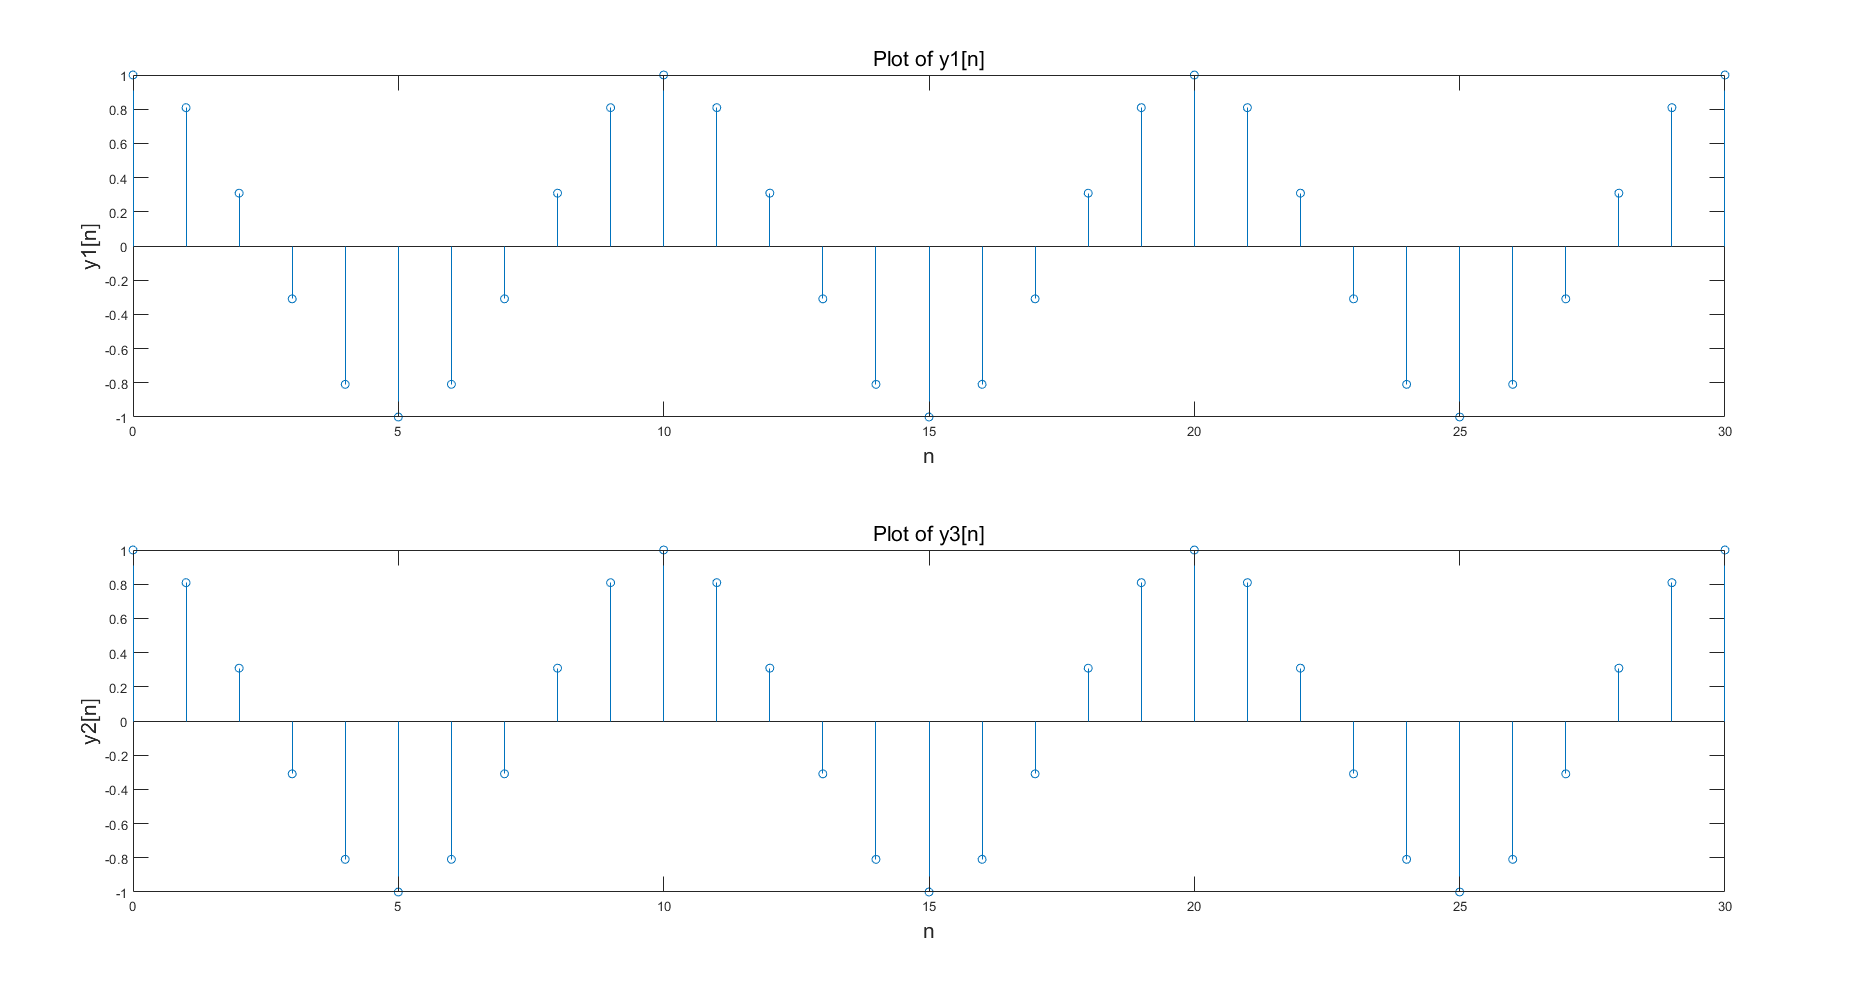
\includegraphics[width=\textwidth]{Question3C.png}

\end{enumerate}

\section{The effects of aliasing in 2D images}

\begin{enumerate}

\item[Q4(a)] Matlab script for reading `barbaraLarge.jpg' into an array. 
\begin{lstlisting}[language=Matlab]
Img = imread('barbaraLarge.jpg');
\end{lstlisting}

\item[Q4(b)] Plot of the image and Matlab script
\begin{lstlisting}[language=Matlab]
Img = imread('barbaraLarge.jpg');
figure,  imshow(Img); title('Original Barbara Image'), colorbar;
\end{lstlisting}

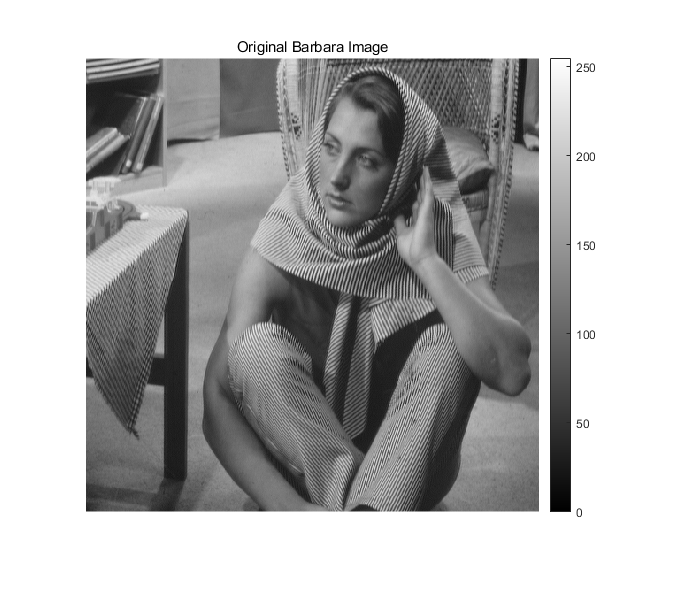
\includegraphics[width=\textwidth]{og.png}
 
\item[Q4(c)] Matlab script. When the image was scaled by a factor of 0.9, there was 
no too much difference between using anti-aliasing and not using anti-aliasing. Also, 
the image still kept relatively enough details / information of the original image. 

When the image was scaled by a factor of 0.7, the regions with a lot of fine lines 
or edges (pants, scarf, tablecloth and the chair) started to lose its details. 
Distortion also started to appear in that region. There was a little bit of 
difference between using anti-aliasing and not using anti-aliasing. Particularly, 
anti-aliasing was applied around woman's knee and lower part of the pants. The 
pixels around those region were become brighter after some black pixels were removed.

When the image was scaled by a factor of 0.5, the image lost a lots of detail and 
the high frequency region distore significantly. Anti-aliasing was applied mainly 
around the scarf, the pants, tablecloth and the chair. Those high frequency region 
looked closer to low frequency region, i.e, the pixels, with darker brightness 
compared to the surrounding pixels, becomre brighter.

\begin{lstlisting}[language=Matlab]
% Running in a debugger, put breakpoint on imshow() function to stop and compare results
resize_factor = [0.9, 0.7, 0.5];
for i = resize_factor(1:3)
    resizeImg = imresize(Img, i, 'nearest', 'antialiasing', 0);
    resizeImgAA = imresize(Img, i, 'nearest', 'antialiasing', 1);
    str = sprintf('Barbara Image resized by %f of original size without anti-aliasing', i);
    strA = sprintf('Barbara Image resized by %f of original size with anti-aliasing', i);
    figure, imshow(resizeImg); title(str), colorbar;
    figure, imshow(resizeImgAA); title(strA), colorbar;
end
\end{lstlisting}

\item[Q4(d)] When the image was reszied by a factor of 0.9, the high frequency 
region, particularly, the pants started showing aliasing. Also, the shadows of 
the table legs also showed small degree of alias. As resizing factor decreased, 
aliasing at the high frequency region (pants, scarf and tablecloth) became 
more obvious. 

In 2D images, the number of pixels and the brightness pixels contain the information 
of the images. Thus, they can be called as the samples of the image. Reszing the 
image to smaller resolution was equivalently reducing the number of pixels from the 
original image, which also meant that the number of samples was reduced, and 
the sampling freuqency was also reduced. Consequently, this generated aliasing 
in the high frequency region due to which the sampling frequency was lower than 
the frequency in high frequency region, as well as the reduce in number of samples.

The regions marked by white shape are the regions that produce aliasing as the 
sample rate decrease

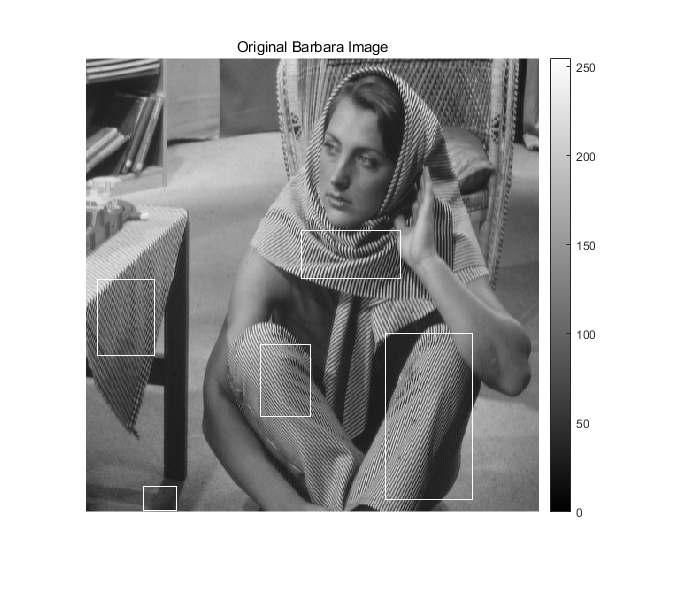
\includegraphics[width=\textwidth]{highlighted.png}

\item[Q4(e)] test3.m demonstration

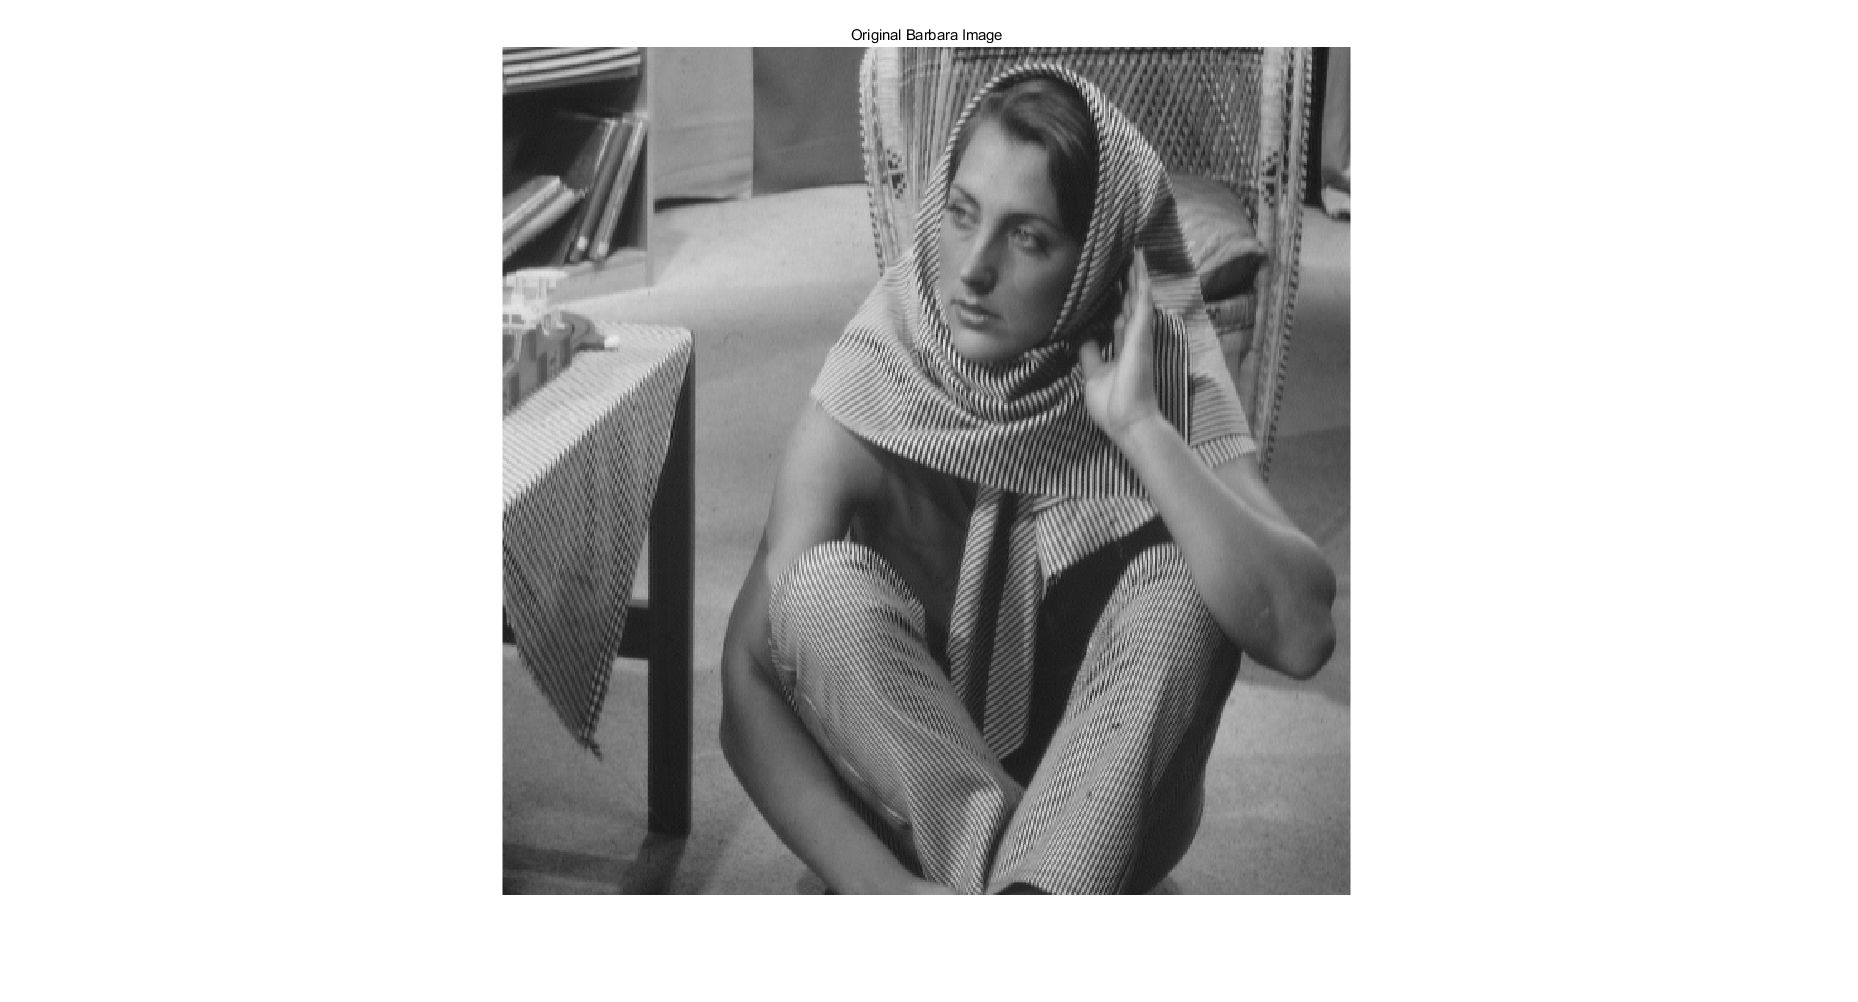
\includegraphics[width=\textwidth]{ognobar.png}
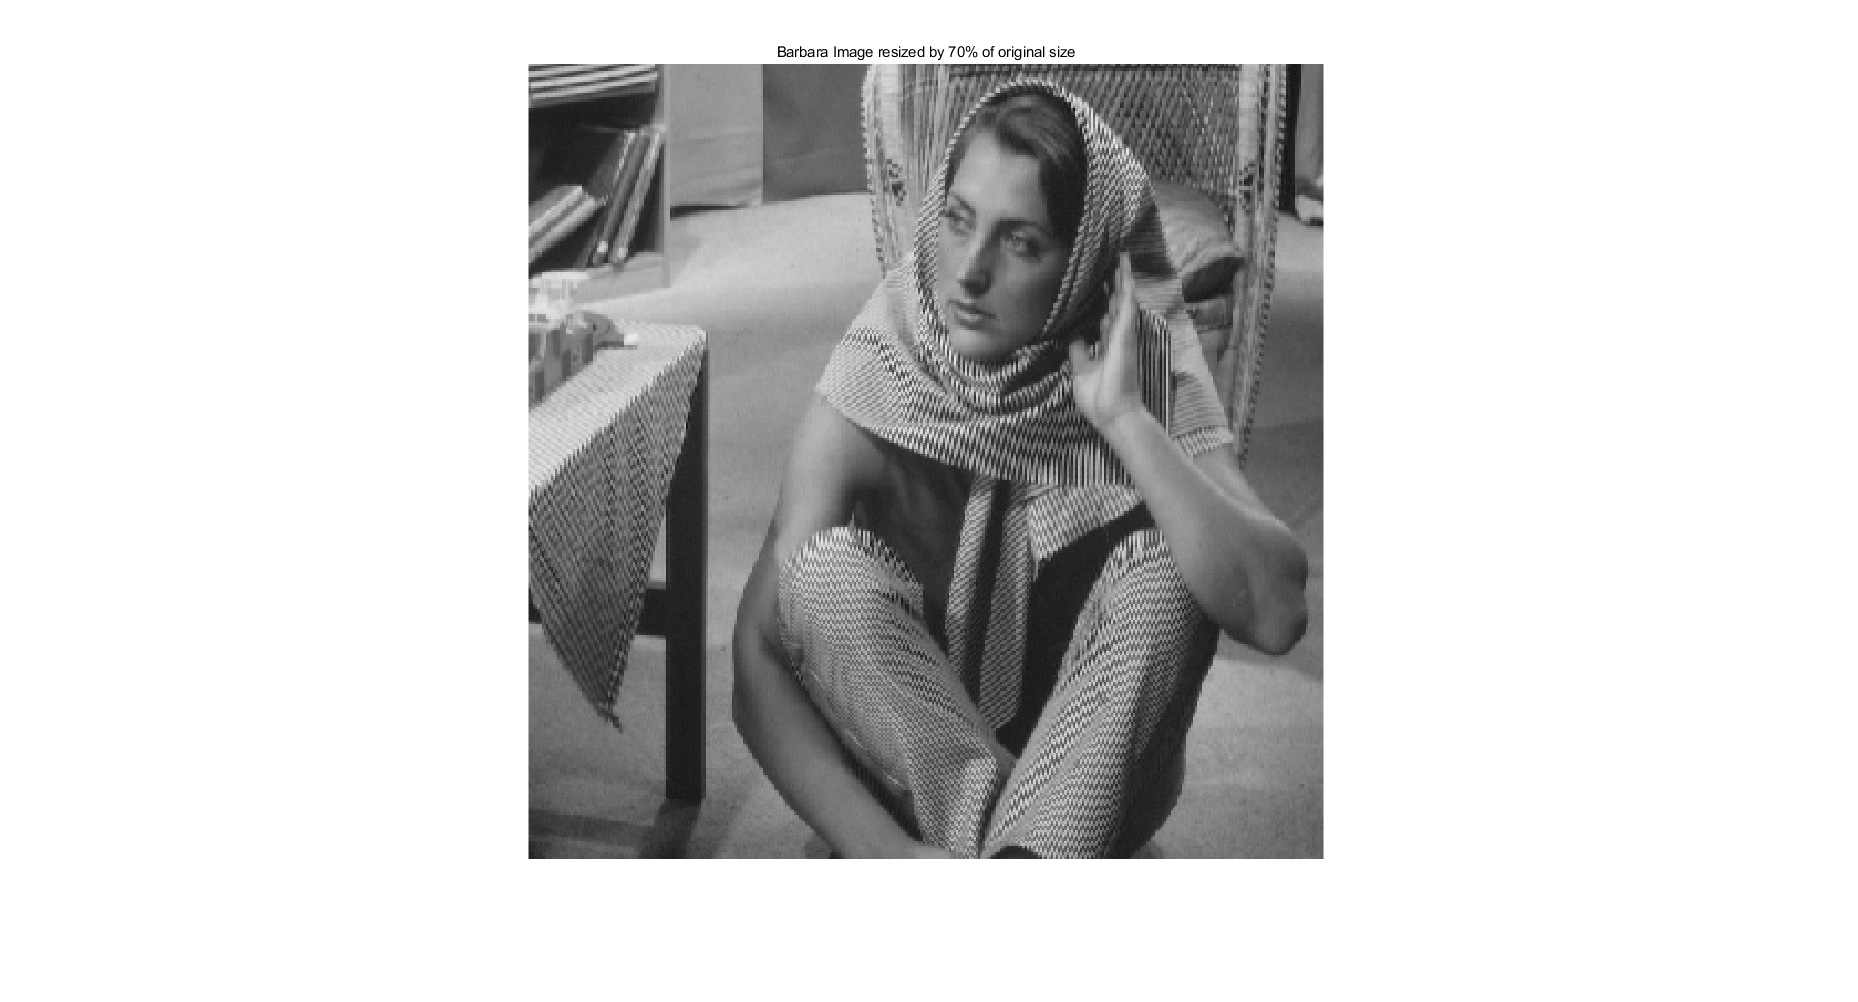
\includegraphics[width=\textwidth]{0.7noLPF.png}
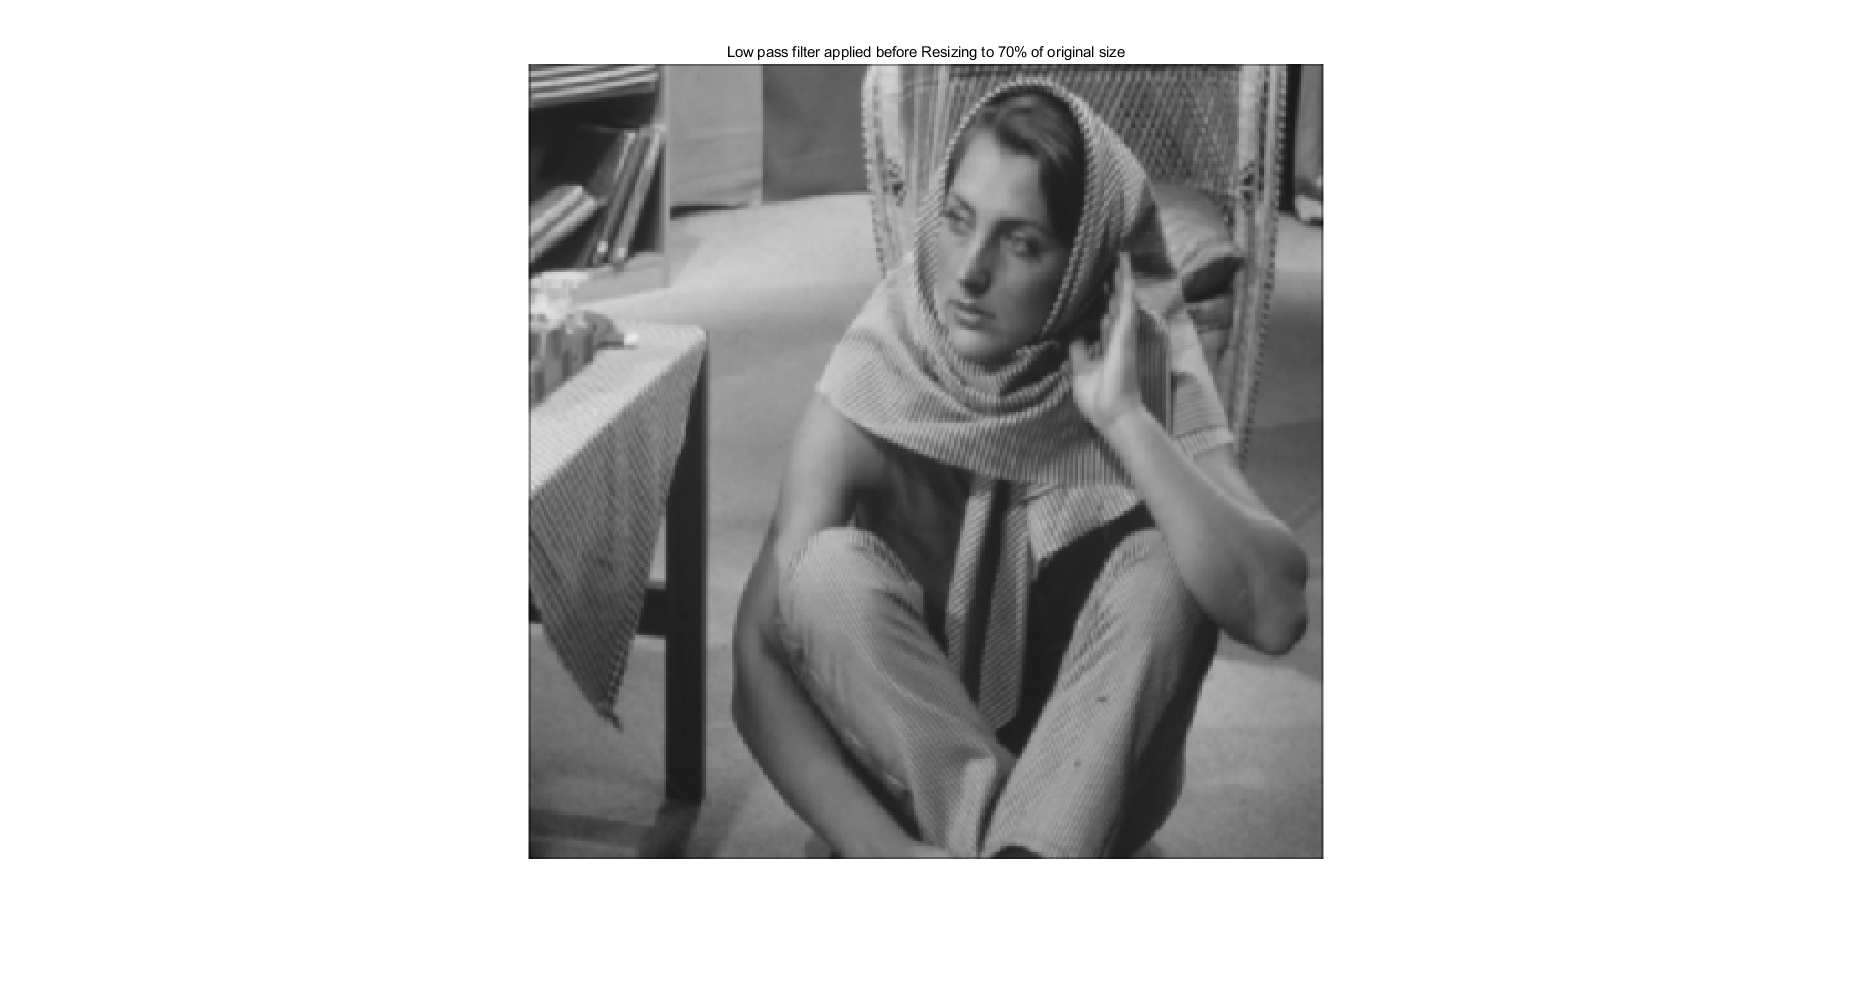
\includegraphics[width=\textwidth]{0.7LPF.png}

\end{enumerate}


\end{document}